%%%%%%%%%%%%%%%%%%%%%%%%%%%%%%%%%%%%%%%%%%%%%%%%%%%%%%%%%%%%%%%%%%%%%%%%%%%%%
%% Original default rstudio/pandoc latex file
%% upated by @jhollist 09/15/2014
%% inspired by @cboetting https://github.com/cboettig/template and
%% @rmflight blog posts:
%% http://rmflight.github.io/posts/2014/07/analyses_as_packages.html 
%% http://rmflight.github.io/posts/2014/07/vignetteAnalysis.html).  
%%%%%%%%%%%%%%%%%%%%%%%%%%%%%%%%%%%%%%%%%%%%%%%%%%%%%%%%%%%%%%%%%%%%%%%%%%%%%

\documentclass[11pt,]{article}
\usepackage[T1]{fontenc}
\usepackage{lmodern}
\usepackage{amssymb,amsmath}
\usepackage{ifxetex,ifluatex}
\usepackage{fancyhdr}
\usepackage{fixltx2e} % provides \textsubscript
% use upquote if available, for straight quotes in verbatim environments
\IfFileExists{upquote.sty}{\usepackage{upquote}}{}
\ifnum 0\ifxetex 1\fi\ifluatex 1\fi=0 % if pdftex
  \usepackage[utf8]{inputenc}
\else % if luatex or xelatex
  \ifxetex
    \usepackage{mathspec}
    \usepackage{xltxtra,xunicode}
  \else
    \usepackage{fontspec}
  \fi
  \defaultfontfeatures{Mapping=tex-text,Scale=MatchLowercase}
  \newcommand{\euro}{€}
\fi
% use microtype if available
\IfFileExists{microtype.sty}{\usepackage{microtype}}{}
\usepackage{longtable,booktabs}
\usepackage{graphicx}
% Redefine \includegraphics so that, unless explicit options are
% given, the image width will not exceed the width of the page.
% Images get their normal width if they fit onto the page, but
% are scaled down if they would overflow the margins.
\makeatletter
\def\ScaleIfNeeded{%
  \ifdim\Gin@nat@width>\linewidth
    \linewidth
  \else
    \Gin@nat@width
  \fi
}
\makeatother
\let\Oldincludegraphics\includegraphics
{%
 \catcode`\@=11\relax%
 \gdef\includegraphics{\@ifnextchar[{\Oldincludegraphics}{\Oldincludegraphics[width=\ScaleIfNeeded]}}%
}%
\ifxetex
  \usepackage[setpagesize=false, % page size defined by xetex
              unicode=false, % unicode breaks when used with xetex
              xetex]{hyperref}
\else
  \usepackage[unicode=true]{hyperref}
\fi
\hypersetup{breaklinks=true,
            bookmarks=true,
            pdfauthor={},
            pdftitle={Modeling Lake Trophic State: A Random Forest Approach},
            colorlinks=true,
            citecolor=blue,
            urlcolor=blue,
            linkcolor=magenta,
            pdfborder={0 0 0}}
\urlstyle{same}  % don't use monospace font for urls
\setlength{\parindent}{0pt}
\setlength{\parskip}{6pt plus 2pt minus 1pt}
\setlength{\emergencystretch}{3em}  % prevent overfull lines
\setcounter{secnumdepth}{5}

%%%%%%%%%%%%%%%%%%%%%%%%%%%%%%%%%%%%%%%%%%%%%%%%%%%%%%%%
%Changes borrowed from @cboettig, added by @jhollist 
% A modified page layout 
\textwidth 6.75in
\oddsidemargin -0.15in
\evensidemargin -0.15in
\textheight 9in
\topmargin -0.5in
\usepackage{lineno} % add 
  \linenumbers % turns line numbering on 
%%%%%%%%%%%%%%%%%%%%%%%%%%%%%%%%%%%%%%%%%%%%%%%%%%%%%%%%

%%%%%%%%%%%%%%%%%%%%%%%%%%%%%%%%%%%%%%%%%%%%%%%%%%%%%%%%
%%Packages and layout changes by @jhollist 09/15/2014
\usepackage{ragged2e}
\usepackage[font=normalsize]{caption}
  \usepackage[doublespacing]{setspace}
\usepackage{parskip}
\usepackage{fancyhdr}
\pagestyle{fancy}
\fancyhf{}
\renewcommand{\headrulewidth}{0pt}
\rfoot{\today}
\lfoot{\thepage}
%%Changed default abstract width and added lines
\renewenvironment{abstract}{
  \hfill\begin{minipage}{1\textwidth}
  \rule{\textwidth}{1pt}\vspace{5pt}
  \normalsize
  \begin{justify}
  \bfseries\abstractname\vspace{5pt}
  \end{justify}}
  {\par\noindent\rule{\textwidth}{1pt}\end{minipage}
}
%%%%%%%%%%%%%%%%%%%%%%%%%%%%%%%%%%%%%%%%%%%%%%%%%%%%%%%%

\title{Modeling Lake Trophic State: A Random Forest Approach}
\author{
Jeffrey W. Hollister
W. Bryan Milstead
Betty J. Kreakie
}
\date{}

\begin{document}
%%Edited by @jhollist 09/15/2014
%%Adds title from YAML
\begin{singlespace}
\begin{center}
\huge Modeling Lake Trophic State: A Random Forest Approach
\end{center}
\rhead{Running head: Modeling Lake Trophic State}
%%Adds Author, correspond email asterisk, and affilnum from YAML
\begin{center}
\large
Jeffrey W. Hollister \textsuperscript{*} \textsuperscript{1} 
W. Bryan Milstead \textsuperscript{1} 
Betty J. Kreakie \textsuperscript{1} 
\end{center}
%%Adds affiliations from YAML
\begin{justify}
\footnotesize \emph{ 
\\*
\textsuperscript{1}US Environmental Protection Agency, Office of Research and Development,
National Health and Environmental Effects Research Laboratory, Atlantic
Ecology Division, 27 Tarzwell Drive Narragansett, RI, 02882, USA\\*
}
%%Adds corresponding author email(s) from YAML
\newcounter{num}
\setcounter{num}{1}
\\[0.1cm]
\footnotesize \emph{ 
\ifnum\value{num}=1%
\textsuperscript{*} corresponding author:
\fi
\href{mailto:hollister.jeff@epa.gov}{\nolinkurl{hollister.jeff@epa.gov}}
\stepcounter{num}
}
\end{justify}
%%Adds date from YAML
\normalsize

\end{singlespace}


\singlespace

\vspace{2mm}

\hrule

\textbf{Abstract}\\Productivity of lentic ecosystems is well studied and
it is widely accepted that as nutrient inputs increase, productivity
increases and lakes transition from lower trophic state
(e.g.~oligotrophic) to higher trophic states (e.g.~eutrophic). These
broad trophic state classifications are good predictors of ecosystem
condition, services, and disservices (e.g.~recreation, aesthetics, and
harmful algal blooms). While the relationship between nutrients and
trophic state provides reliable predictions, it requires \emph{in situ}
water quality data in order to parameterize the model. This limits the
application of these models to lakes with existing and, more
importantly, available water quality data. To predict trophic state in
lakes without water quality data, we take advantage of the availability
of a large national lakes water quality database (i.e.~the National
Lakes Assessment), land use/land cover data, lake morphometry data,
other universally available data, and apply modern data mining
approaches to build and assess models of lake trophic state. We use
random forests and random forest variable selection to identify
variables to be used for predicting trophic state and we compare the
performance of two sets of models of chlorophyll \emph{a} derived
trophic state. The first set of models estimates three different trophic
state classification with both \emph{in situ} and universally available
data. The second set of models uses universally available GIS data only.
Overall accuracy for models built from \emph{in situ} and universal data
ranged from 67\% to 87\%. For the universal data only models, overall
accuracy ranged from 49\% to 76\%. Lastly, presence and abundance of
cyanobacteria is often strongly associated with trophic state. To test
this we examine the association between estimates of cyanobacteria
abundance and measured chlorophyll \emph{a} and find a positive
relationship. We find, that predictive models of lake trophic state may
be improved with additional information on the landscape surrounding
lakes and that those models provide additional information on the
presence of potentially harmful cyanobacteria taxa. Lastly, the source
code and data for this manuscript are available from
\url{https://github.com/USEPA/LakeTrophicModelling}.

\vspace{3mm}

\hrule

\doublespace

\section{Introduction}\label{introduction}

Productivity in lentic systems is often categorized across a range of
trophic states (e.g.~the trophic continuum) from early successional
(i.e.~oligotrophic) to late successional lakes (i.e.~hypereutrophic)
with lakes naturally occurring across this range (Carlson 1977).
Oligotrophic lakes occur in nutrient poor areas or have a more recent
geologic history, are often found in higher elevations, have clear
water, and are usually favored for drinking water or direct contact
recreation (e.g.~swimming). Lakes with higher productivity
(e.g.~mesotrophic and eutrophic lakes) have greater nutrient loads, tend
to be less clear, have greater density of aquatic plants, and often
support more diverse and abundant fish communities. Higher primary
productivity is not necessarily a predictor of poor ecological condition
as it is natural for lakes to shift from lower to higher trophic states
but this is a slow process. However, at the highest productivity levels
(hypereutrophic lakes) biological integrity is compromised (Hasler 1969,
Smith et al. 1999, Schindler and Vallentyne 2008).

Monitoring trophic state allows the identification of rapid shifts in
trophic state or locating lakes with unusually high productivity
(e.g.~hypereutrophic). These cases are indicative of lakes under greater
anthropogenic nutrient loads, also known as cultural eutrophication, and
are more likely to be at risk of fish kills, fouling, and harmful algal
blooms (Smith 1998, Smith et al. 1999, 2006). Given the association
between trophic state and many ecosystem services and disservices, being
able to accurately model trophic state could provide a first cut at
identifying lakes with the potential for harmful algal blooms (i.e.~from
cyanobacteria) or other problems associated with cultural
eutrophication. This type of information could be used for setting
priorities for managment and allow for more effecient use of limited
resources.

As trophic state and related indices can be best defined by a number of
\emph{in situ} water quality parameters (modeled or measured), most
models have used this information as predictors (Imboden and G{ä}chter
1978, Salas and Martino 1991, Carvalho et al. 2011, Milstead et al.
2013). This leads to accurate models, but also requires data that are
often sparse and not always available, thus limiting the population of
lakes for which we can make predictions. A possible solution for this is
to build models that use widely available data that are correlated to
many of the \emph{in situ} variables. For instance, landscape metrics of
forests, agriculture, wetlands, and urban land in contributing
watersheds have all been shown to explain a significant proportion of
the variation (ranging from 50-86\%, depending on study) in nutrients in
receiving waters (Jones et al. 2001, 2004, Seilheimer et al. 2013).
Building on these previously identified associations might allow us to
use only landscape and other universally available data to build models.
Identifying predictors using this type of ubiquitous data would allow
for estimating trophic state in both monitored and unmonitored lakes.

Many published models of nutrients and trophic state in freshwater
systems are based on linear modelling methods such as standard least
squares regression or linear mixed models (Jones et al. 2001, 2004).
While these methods have proven to be reliable, they have limitations
(e.g.~independence and distribution assumptions, and outlier
sensitivity). Using data mining approaches, such as random forests,
avoids many of the limitations, may reduce bias and often provides
better predictions (Breiman 2001, Cutler et al. 2007, Peters et al.
2007). For instance, random forests are non-parametric and thus the data
do not need to come from a specific distribution (e.g.~Gaussian) and can
contain collinear variables (Cutler et al. 2007). Second, random forests
work well with very large numbers of predictors (Cutler et al. 2007).
Lastly, random forests can deal with model selection uncertainty as
predictions are based upon a consensus of many models and not just a
single model selected with some measure of goodness of fit.

To build on past work, we have identified five areas in which this
research contributes. First, we update trophic state modelling efforts
with the use of random forests. Second, we assess the accuracy of
predicted trophic state in lakes with the a) \emph{in situ} and
universally available GIS data and then b) with the universally
available GIS data only. Third, we identify important variables for
describing lake trophic state. Fourth, we explore associations between
trophic state and cyanobacteria, a key taxa in harmful algal blooms, so
that we may begin to understand how changes in trophic state may be
linked to an important ecosystem disservice. Lastly, a key goal of this
research is to provide full access to the data and code. As such, this
paper, the code, and the data used in the models is made available as an
R package from \url{https://github.com/USEPA/LakeTrophicModeling}.

\section{Methods}\label{methods}

\subsection{Data and Study Area}\label{data-and-study-area}

We utilize three primary sources of data for this study, the National
Lakes Assessment (NLA), the National Land Cover Dataset (NLCD), and lake
morphometery modeled from the NHDPlus and National Elevation Data Set
(Homer et al. 2004, USEPA 2009, Xian et al. 2009, Hollister and Milstead
2010, Hollister et al. 2011, Hollister 2014). All datasets are national
in scale and provide a unique snapshot view of the condition of lakes in
the conterminous United States during the summer of 2007.

The NLA data were collected during the summer of 2007 and the final data
were released in 2009 (USEPA 2009). With consistent methods and metrics
collected at 1056 locations across the conterminous United States
(Figure \ref{fig:nlaMap}), the NLA provides a unique opportunity to
examine broad scale patterns in lake productivity. The NLA collected
data on biophysical measures of lake water quality and habitat as well
as an assessment of the phytoplankton community. For this analysis we
examined the water quality measurements and total cyanobacteria
abundance from the National Lakes Assessment (USEPA 2009).

Adding to the monitoring data collected via the NLA, we use the 2006
NLCD data to examine landscape-level drivers of trophic status in lakes.
The NLCD is a national land use/land cover dataset that also provides
estimates of impervious surface. We calculated total proportion of each
NLCD land use land cover class and total percent impervious surface
within a 3 kilometer buffer surrounding each lake (Homer et al. 2004,
Xian et al. 2009). A three kilometer buffer was selected as an
intermediate measure of the adjacent neighborhood; the three kilometer
buffer size is greater than the immediate parcel but smaller than
regional and whole-basin measures.

To account for unique aspects of each lake and characterize lake
productivity, we also used measures of lake morphometry (i.e.~depth,
volume, fetch, etc.). As these data are difficult to obtain for large
numbers of lakes over broad regions, we used modeled estimates of lake
morphometry (Hollister and Milstead 2010, Hollister et al. 2011,
Hollister 2014). These included: surface area, shoreline length,
Shoreline Development, Maximum Depth, Mean Depth, Lake Volume, Maximum
Lake Length, Mean Lake Width, Maximum Lake Width, and Fetch.

\subsection{Predicting Trophic State with Random
Forests}\label{predicting-trophic-state-with-random-forests}

Random forest is a machine learning algorithm that aggregates numerous
decision trees in order to obtain a consensus prediction of the response
categories (Breiman 2001). Bootstrapped sample data are recursively
partitioned according to a given random subset of predictor variables
and a predetermined number of decision trees are developed. With each
new tree, the sample data subset is randomly selected and with each new
split, the subset of predictor variables are randomly selected. A
detailed discussion of the benefits of a random forest approach is
beyond the scope of this paper. To find out more see Breiman (2001) and
Cutler et al. (2007).

Random forests are able to handle numerous correlated variables without
a decrease in prediction accuracy; however, one possible downfall to
this approach is that the resulting model may be difficult to interpret.
This is a problem often faced in gene selection and in that field, a
variable selection method based on random forest has been successfully
applied and implemented in the R Language as the \texttt{varSelRF}
package (D{í}az-Uriarte and De Andres 2006). With this method, a minimum
set of variables that maximizes model accuracy is provided. This allows
us to start with a full suite of predictor variables from which to
select a minimum, easier to interpret set of variables. One issue with
the approach in \texttt{varSelRF} is that because of the randomization
inherent in random forests it is possible to get variation in the
minimum selected set of variables. To account for this we repeated
\texttt{varSelRF} 100 times. In our case, repeating the procedure 100
times quickly converged on a set of all possible important variables.

\subsection{Model Details}\label{model-details}

Using both the \texttt{varSelRF} and \texttt{randomForest} R packages we
ran models for six sets of variables and trophic state classifications
(Liaw and Wiener 2002, Diaz-Uriarte 2010). These included three
different combinations of the chlorophyll \emph{a} trophic states as the
dependent variables and using all variables (\emph{in situ} and GIS
variables) or the GIS only variables (i.e.~no \emph{in situ}
information) as the independent variables in the random forest. A
listing of all considered variables is in Appendix 1. Trophic state was
defined using the NLA chlorophyll \emph{a} trophic state cut offs and
the three combinations of trophic state were used to highlight the
possible error caused by misclassification of adjacent classes, such as
mesotrophic and eutrophic (Table \ref{tab:trophicStateTable}). Our
separation of predictors was chosen so that we could highlight the
additional predictive performance provided by adding the \emph{in situ}
water quality variables on top of the GIS only variables. Lastly, we
used only complete cases (i.e.~missing data were removed) so the total
number of observations varied between models.

The six model combinations were:

\begin{itemize}
\itemsep1pt\parskip0pt\parsep0pt
\item
  \textbf{Model 1:} Chlorophyll \emph{a} trophic state (4 class) = All
  variables (\emph{in situ} water quality, lake morphometry, and
  landscape)
\item
  \textbf{Model 2:} Chlorophyll \emph{a} trophic state (3 class) = All
  variables (\emph{in situ} water quality, lake morphometry, and
  landscape)
\item
  \textbf{Model 3:} Chlorophyll \emph{a} trophic state (2 class) = All
  variables (\emph{in situ} water quality, lake morphometry, and
  landscape)
\item
  \textbf{Model 4:} Chlorophyll \emph{a} trophic state (4 class) = GIS
  Only variables (lake morphometry, and landscape)
\item
  \textbf{Model 5:} Chlorophyll \emph{a} trophic state (3 class) = GIS
  Only variables (lake morphometry, and landscape)
\item
  \textbf{Model 6:} Chlorophyll \emph{a} trophic state (2 class) = GIS
  Only variables (lake morphometry, and landscape)
\end{itemize}

Our modelling work flow was as follows:

\begin{enumerate}
\def\labelenumi{\arabic{enumi}.}
\itemsep1pt\parskip0pt\parsep0pt
\item
  Use \texttt{iterVarSelRF} in the \texttt{LakeTrophicModelling} R
  package to identify a minimal set of variables that maximize accuracy
  of the random forest algorithm (Diaz-Uriarte 2010, Hollister et al.
  2014). This subset of variables, the reduced model, is calculated for
  each of our 6 models.
\item
  Using R's \texttt{randomForest} package, we pass the reduced models
  selected with \texttt{iterVarSelRF} and assess model performance (Liaw
  and Wiener 2002).
\end{enumerate}

\subsection{Measures of Model Performance and Variable
Importance}\label{measures-of-model-performance-and-variable-importance}

We assessed the performance of the random forest models by comparing the
total prediction accuracy and the kappa coefficient of the final
confusion matrix. For each of the models, the final predictions were
compared to the original data via a confusion matrix. A confusion matrix
shows agreement and disagreement with predicted values forming the
columns of the matrix and observed values, the rows. The total accuracy
(i.e.~percent correctly predicted) was calculated. Since some agreement
can be expected by chance alone, it is also useful to take this type of
error into account. For this we calculated the kappa coefficient from
the confusion matrix for each model as well (Cohen 1960, Hubert and
Arabie 1985). The kappa coefficient can range from -1 to 1 with 0
equalling the agreement expected by chance alone. Values greater than 0
represent agreement greater than would be expected by chance, with
values greater than 0.61 considered ``substantial'' agreement (Landis
and Koch 1977). Negative values are rare and would indicate no agreement
between the predicted and observed values. Additonally, random forest
builds each tree on bootstrapped, random subsets of the original data,
thus, a separate independent validation dataset is not required and
random forest error estimates are expected to be unbiased (Breiman
2001).

Lastly, the random forest algorithm explicitly measures variable
importance as mean decrease in Gini. The Gini Index is a measure of how
well the data are classified into homogeneous groups. For every node,
the splitting variables are permuted and the change in actual Gini and
permuted Gini is recorded. The mean decrease Gini is a summed and
standardized value for each variable (Breiman 2001). Higher values of
mean decrease Gini suggest a higher importance for that variable.

\section{Results}\label{results}

Our complete dataset includes 1148 lakes; however 5 lakes did not have
chlorophyll \emph{a} data. Thus, the base dataset for our modelling was
conducted on data for 1143 lakes. As chlorophyll \emph{a} is used to
create the trophic state classifications, it was necessary to remove
these data because no chlorophyll \emph{a} trophic state could be
determined for these lakes. The lakes were well distributed both across
the four trophic state categories (Table \ref{tab:trophicStateTable})
and spatially throughout the United States (Figure \ref{fig:nlaMap}).

\subsection{Models}\label{models}

Accuracy for the models built with all predictors ranged from 67\% to
87\% and the kappa coefficient had a minimum value of 0.55 and maximum
of 0.73. The GIS only models had a total accuracy between 49\% and 76\%
and kappa coefficient between 0.3 and 0.52. The importance of variables
for the models including the \emph{in situ} data were fairly stable
while there was considerably more variation in variable importance for
the three different GIS only models. Additionally, as each model
contained a different subset of variables and since we removed
observations with missing data, the total number of lakes varied across
the models. Details for each model are discussed below.

\emph{Model 1: 4 Trophic States \textasciitilde{} All Variables}

Total number of lakes for Model 1 was 1142 and the reduced model for
Model 1 included turbidity, total phosphorus, total nitrogen,
nitrogen:phosphorus ratio, total organic carbon, potassium, ecoregion,
maximum depth, organic ions, and dissolved organic carbon. Of these,
turbidity, total phosphorus, and total nitrogen were the three most
important predictors of the four classes of trophic state (Figure
\ref{fig:Importance_Model1}). Total accuracy for Model 1 was 67\% and
the Cohen's Kappa was 0.55 (Table \ref{tab:Confusion_Model1}).

\emph{Model 2: 3 Trophic States \textasciitilde{} All Variables}

For Model 2 there were 1130 observations and the reduced model included
turbidity, total phosphorus, total nitrogen, total organic carbon,
nitrogen:phosphorus, longitude, pH, estimated organic anions, elevation,
maximum depth, dissolved organic carbon, potassium, latitude, ecoregion,
chloride, ammonium and percent cropland (Figure
\ref{fig:Importance_Model2}). The top predictors for 3 trophic state
classes were again turbidity, total phosphorus, and total nitrogen
(Figure \ref{fig:Importance_Model2}). Model 2 accuracy was 80\% and the
Cohen's Kappa was 0.61 (Table \ref{tab:Confusion_Model2}).

\emph{Model 3: 2 Trophic States \textasciitilde{} All Variables}

Model 3 was built with 1142 lakes and the reduced model was similar to
Model 1 and Model 2. This model included turbidity, total phosphorus,
total nitrogen, nitrogen:phosphorus, potassium, ecoregion, elevation,
total organic carbon, growing degree days, longitude, sodium, maximum
depth, estimated organic anions, latitude, and dissolved organic carbon
(Figure \ref{fig:Importance_Model3}). The top three predictors were the
same as Models 1 and 2. (Figure \ref{fig:Importance_Model3}). Total
accuracy for Model 3 was 87\% and the Cohen's Kappa was 0.73 (Table
\ref{tab:Confusion_Model3}).

\emph{Model 4: 4 Trophic States \textasciitilde{} GIS Only Variables}

Model 4 had a sample size of 1138. The selected variables for the Model
4 were longitude, latitude, elevation, estimated mean lake depth,
percent evergreen forest, estimated maximum lake depth, percent
cropland, and ecoregion (Figure \ref{fig:Importance_Model4}). The three
most important variables were longitude, latitude, and elevation (Figure
\ref{fig:Importance_Model4}); however, all variables except ecoregion
were almost equally important. Total accuracy for Model 4 was 49\% and
the Cohen's Kappa was 0.3 (Table \ref{tab:Confusion_Model4}).

\emph{Model 5: 3 Trophic States \textasciitilde{} GIS Only Variables}

A total of 1138 lakes were used for model 5 which included estimated
mean lake depth, percent cropland, longitude, latitude, percent
evergreen forest, elevation, estimated maximum lake depth, estimated
lake volume, percent deciduous forest, percent developed open space,
ecoregion, percent woody wetland, and percent shrub/scrub (Figure
\ref{fig:Importance_Model5}). The most important variables for model 5
were estimated mean lake depth, percent cropland, and longitude. (Figure
\ref{fig:Importance_Model5}). Total accuracy for Model 5 was 68\% and
the Cohen's Kappa was 0.35 (Table \ref{tab:Confusion_Model5}).

\emph{Model 6: 2 Trophic States \textasciitilde{} GIS Only Variables}

Model 6 was built using 1138 total observations. The variable selection
process for Model 6 produced a reduced model with ecoregion, growing
degree days, percent evergreen forest, percent cropland, elevation,
estimated mean lake depth, longitude, latitude, watershed area,
estimated maximum lake depth, percent developed open space, percent
deciduous forest, and estimated lake volume (Figure
\ref{fig:Importance_Model6}). The three most important variables were
ecoregion, growing degree days, and percent evergreen. (Figure
\ref{fig:Importance_Model6}). Ecoregion had the highest importance with
a slow decline in importance for the remainder of the variables. Total
accuracy for Model 6 was 76\% and the Cohen's Kappa was 0.52 (Table
\ref{tab:Confusion_Model6}).

\section{Discussion}\label{discussion}

\subsection{Trophic State
Probabilities}\label{trophic-state-probabilities}

One of the powerful features of random forests is the ability to
aggregate a very large number of competing models or trees. Each tree
provides an independent prediction or vote for a possible outcome. In
the context of our trophic state models, we have 10,000 votes for each
lake. These values may be interpreted as the probability that a lake is
in a given trophic state. For instance, for a single lake (National Lake
Assessment ID = NLA06608-0005), the vote probabilities for Model 1 were
81\% for oligotrophic, 19\% for mesotrophic, 0\% for eutrophic, and 0\%
for hypereutrophic. This suggests little uncertainty in the predicted
oligotrophic state.

Further, the maximum probability for each lake can be used as a measure
of how certain the random forest model was of the prediction. We would
expect higher total accuracy for lakes that had more certain
predictions. Some lakes may have many votes for a single trophic state
and few votes for other trophic states and these would thus have a large
maximum probability and the random forest predicitions would be more
certain. Alternatively, the 10,000 votes could have been spread more
equally across the trophic state classes for a lake and that lake would
have a small maximum probability and the final predictions would be less
certain. This should be evident by looking at the total classification
accuracy of lakes given their maximum probability is above a certain
point. To test this we can examine the accuracy of trophic state
predictions across the full range of trophic state probabilities,
similar to an approach outlined by Paul and MacDonald (2005) and
implemented by Hollister et al. (2008). We utilize this approach and
examine the change in total accuracy as a function of the maximum
probability for each lake. As expected, lakes with higher maximum vote
probabilities were more accurately predicted (Figure
\ref{fig:condProbFig}). The increasing trend suggests that even for
models with lower overall accuracy there can also be a large number of
individual cases that are predicted with high accuracy.

\subsection{Variable Selection and
Importance}\label{variable-selection-and-importance}

There was a great deal of agreement on the important variables for each
set of models. In line with past predictive modeling of cyanobacteria
abundance and not surprisingly, the \emph{in situ} models consistently
select the water quality variables (turbidity, total nitrogen, total
phosphorus, and N:P ratios) as important variables (Downing et al.
2001). While there is variation in the response of cyanobacteria to
changes in relative nutrient concentrations, the general pattern
suggests that limiting nutrients have considerable impact once amounts
increase beyond expected levels.

The mechanistic role of turbidity on lake trophic state is more complex.
Light availability in turbid waters is lower than in clear waters. This
would suggest a negative relationship between turbidity and chlorophyll
\emph{a}. Second, chlorophyll \emph{a} can also be a component of
turbidity and lakes with higher chlorophyll \emph{a} concentrations will
also be more turbid. Last, chlorophyll \emph{a} is not the only
component of of turbidity and turbid waters can be caused by, for
example, increased sediment loads or tannin. This would be a cause for
concern with linear models; however, linearity is not an assumption of
tree-based modelling approaches such as random forest.

Our models with the GIS-only variables captured the large scale spatial
pattern of the trophic status gradient of lakes across the United
States. We reliably saw latitude and longitude and ecoregion selected as
important variables. It is also possible that other variables selected
as important are also capturing a portion of this trend. For instance,
elevation and growing degree days both have obvious spatial components,
but may also be accounting for variation in temperature.

The land use/land cover variables were also important in describing
trophic state patterns. Like elevation and growing degree days, broad
scale spatial patterns are inherent in the data. For instance, the
relative continental position of mountains in the United States is the
spatial inverse of the distribution of agricultural lands. However, it
is known that forests are positively associated with lower nutrient
loads where as agricultural land shows a negative association. These
more local scale relationships with land use/land cover likely provide
additional predictive power to the information in the broader scale
data.

Lastly, morphometry (e.g.~depth and volume) also proved to be important
in the prediction of lake trophic state. As morphometry shows little to
no broad scale spatial pattern and is unique to a given lake, these data
are likely illuminating the local, lake scale drivers of trophic state.
As only depth and volume were selected, this likely shows the importance
of in-lake nutrient processing and residence time.

\subsection{Associating Trophic State and
Cyanobacteria}\label{associating-trophic-state-and-cyanobacteria}

Cyanobacteria biomass should be closely associated with trophic state as
cyanobacteria contribute to the chlorophyll concentration in a lake. If
these associations are strong enough we may be able to expand models
such as those reported here to also predict probability of cyanobacteria
blooms. To test if trophic state can be used to differentiate
cyanobacteria abundance, we examine distribution of cyanobacteria
abundance for each trophic state and also explored linear associations
between chlorohyll \emph{a} and cyanobacteria abundance.

The distribution of cyanobacteria abundance showed separation between
all of the trophic state classifications (Figures
\ref{fig:ts_4_cyano_cdf}, \ref{fig:ts_3_cyano_cdf}, and
\ref{fig:ts_2_cyano_cdf}) and there was a significant linear
relationship (r\textsuperscript{2}=0.33) between chlorophyll \emph{a}
and cyanobacteria abundance (Figure \ref{fig:scatterplot}). Furthermore,
Yuan et al. (2014) used the 2007 NLA to demonstrate that total nitrogen
and chlorophyll \emph{a} concentrations were good predictors of World
Health Organization microcystin (a toxin produced by some cyanobacteria)
criteria exceedences. These results suggest that trophic state is indeed
an acceptable proxy for cyanobacteria abundance and that in lakes with
higher trophic state it is also reasonable to expect higher
cyanobacteria.

\section{Conclusions}\label{conclusions}

Our research goals were to explore the utility of a widely used data
mining algorithm, random forests, in the modelling of lake trophic
state. Further, we hoped to examine the utility of these models when
built with only ubiquitous GIS data, which allows estimation of trophic
state for all lakes in the United States. We were able to successfully
predict a variety of trophic state classes. With the GIS only models our
total accuracy ranged from 49\% to 76\%, and with the full suite of data
our model accuracy had a minimum accuracy of 67\% and maximum accuracy
of 87\%.

While some of the models (i.e.~Model 4) showed relatively low prediction
accuracies, another feature of the random forest, votes, can provide
additional information. In addition to providing a single estimate of
trophic state for each lake, our models also indicated the probability
that a lake was classified in any of the categories. These probabilities
may be mapped directly to show the uncertainty of a given predicted
class. Furthermore, as the certainty of prediction increases, so does
overall trophic state classification accuracy (Figure
\ref{fig:condProbFig}). These results suggest that our models will
provide reasonable estimates of trophic state across the United States.

There was great deal of agreement on the important variables for each
set of models. For the combined \emph{in situ} and GIS models, the
\emph{in situ} water quality variables drove the predictions. This is
expected. For the GIS only models, the results were more nuanced with
three broad categories routinely being selected as important: broad
scale spatial patterns in trophic state, land use/land cover controls of
trophic state, and local, lake-scale control driven by lake morphometry.
Lastly, associations between trophic state and cyanobacteria showed
that, at the broad scale of the 2007 NLA, there is a linear relationship
between chlorophyll \emph{a} and cyanobacteria abundance and that using
trophic state as a proxy for cyanobacteria has potential.

These broad categories and the association between trophic state and
total cyanobacteria abundance raise three important considerations
related to managing eutrophication. First, the broad scale patterning
suggests regional trends. This is important because it suggests that
efforts to monitor, model and manage eutrophication and cyanobacteria
should be undertaken at both national and regional levels. Second, while
direct control of water quality in lakes would have a large impact, the
land use/land cover drivers (i.e.~non-point sources) of water quality
are also important, and better management of the spatial distribution of
important classes such as forest and agriculture can provide some level
of control on trophic state and amount of cyanobacteria present. Third,
in-lake processes (i.e.~residence time, nutrient cycling, etc.) are, as
expected, very important and need to be part of any management strategy.
Building on these efforts through updated models, direct prediction of
cyanobacteria, and additional information on the regional differences
will help us get a better handle on the broad scale dynamics of
productivity in lakes and the potential risk to human health from
cyanobacteria blooms.

\section{Acknowledgements}\label{acknowledgements}

We would like to thank Farnaz Nojavan, Nathan Schmucker, John Kiddon,
Joe LiVolsi, Tim Gleason, and Wayne Munns for constructive reviews of
this paper. This paper has not been subjected to Agency review.
Therefore, it does not necessary reflect the views of the Agency.
Mention of trade names or commercial products does not constitute
endorsement or recommendation for use. This contribution is identified
by the tracking number ORD-011075 of the Atlantic Ecology Division,
Office of Research and Development, National Health and Environmental
Effects Research Laboratory, US Environmental Protection Agency.

\newpage

\section{Figures}\label{figures}

\begin{figure}[htbp]
\centering
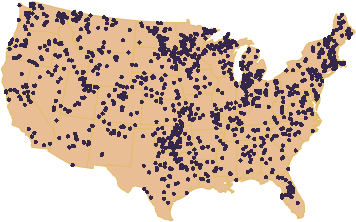
\includegraphics{manuscript_files/figure-latex/nlaMap-1.jpeg}
\caption{Map of the distribution of National Lakes Assesment Sampling
locations\label{fig:nlaMap}}
\end{figure}

\newpage

\begin{figure}[htbp]
\centering
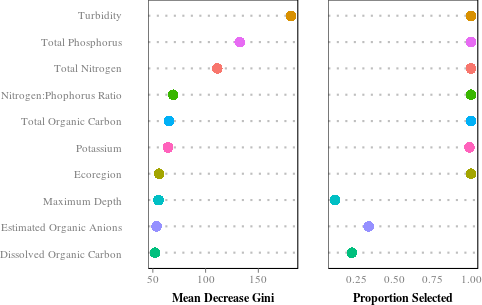
\includegraphics{manuscript_files/figure-latex/Importance_Model1-1.jpeg}
\caption{Importance plot for Model 1, shows mean descrease gini and
proportion of times a variable was selected for inclusion in the model.
Higher values of mean decrease gini indicate higher importance.
\label{fig:Importance_Model1}}
\end{figure}

\newpage

\begin{figure}[htbp]
\centering
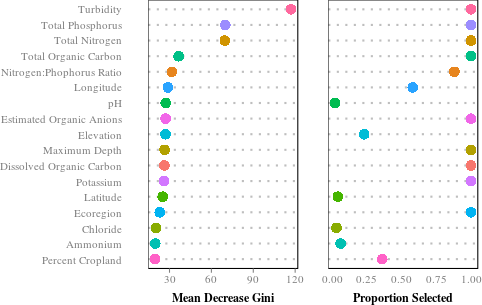
\includegraphics{manuscript_files/figure-latex/Importance_Model2-1.jpeg}
\caption{Importance plot for Model 2, shows mean descrease gini and
proportion of times a variable was selected for inclusion in the model.
Higher values of mean decrease gini indicate higher importance.
\label{fig:Importance_Model2}}
\end{figure}

\newpage

\begin{figure}[htbp]
\centering
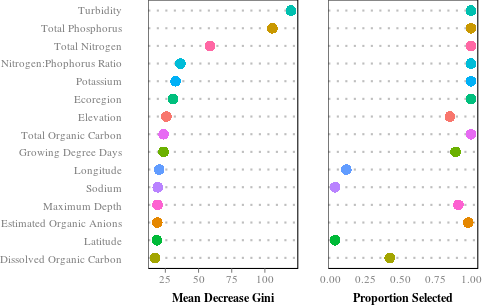
\includegraphics{manuscript_files/figure-latex/Importance_Model3-1.jpeg}
\caption{Importance plot for Model 3, shows mean descrease gini and
proportion of times a variable was selected for inclusion in the model.
Higher values of mean decrease gini indicate higher importance.
\label{fig:Importance_Model3}}
\end{figure}

\newpage

\begin{figure}[htbp]
\centering
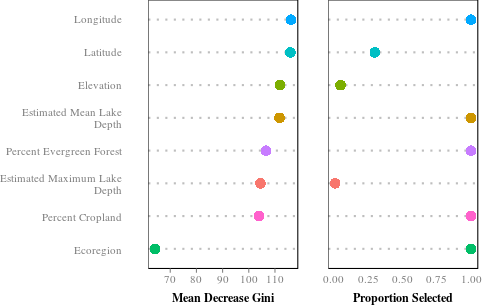
\includegraphics{manuscript_files/figure-latex/Importance_Model4-1.jpeg}
\caption{Importance plot for Model 4, shows mean descrease gini and
proportion of times a variable was selected for inclusion in the model.
Higher values of mean decrease gini indicate higher importance.
\label{fig:Importance_Model4}}
\end{figure}

\newpage

\begin{figure}[htbp]
\centering
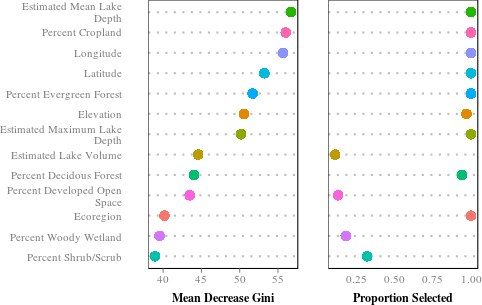
\includegraphics{manuscript_files/figure-latex/Importance_Model5-1.jpeg}
\caption{Importance plot for Model 5, shows mean descrease gini and
proportion of times a variable was selected for inclusion in the model.
Higher values of mean decrease gini indicate higher importance.
\label{fig:Importance_Model5}}
\end{figure}

\newpage

\begin{figure}[htbp]
\centering
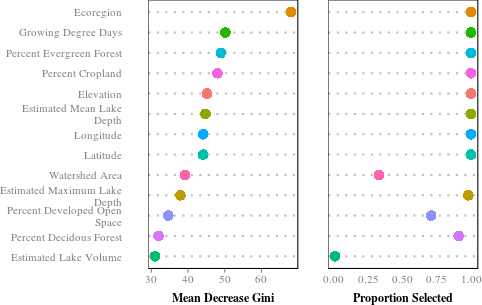
\includegraphics{manuscript_files/figure-latex/Importance_Model6-1.jpeg}
\caption{Importance plot for Model 6, shows mean descrease gini and
proportion of times a variable was selected for inclusion in the model.
Higher values of mean decrease gini indicate higher importance.
\label{fig:Importance_Model6}}
\end{figure}

\newpage

\begin{figure}[htbp]
\centering
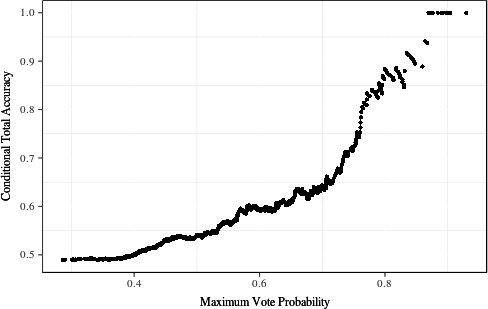
\includegraphics{manuscript_files/figure-latex/condProbFig-1.jpeg}
\caption{Comparison of certainity of trophic state prediction and total
accuracy\label{fig:condProbFig}}
\end{figure}

\newpage

\begin{figure}[htbp]
\centering
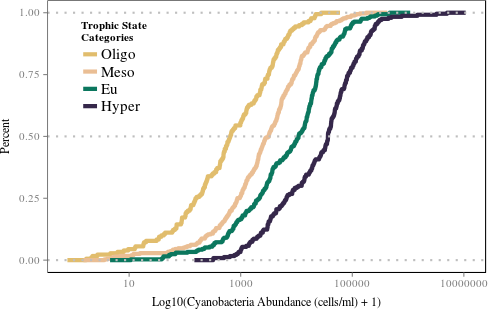
\includegraphics{manuscript_files/figure-latex/ts_4_cyano_cdf-1.jpeg}
\caption{Cumulative distribution function of cyanobacetria abundance for
4 trophic state classes\label{fig:ts_4_cyano_cdf}}
\end{figure}

\newpage

\begin{figure}[htbp]
\centering
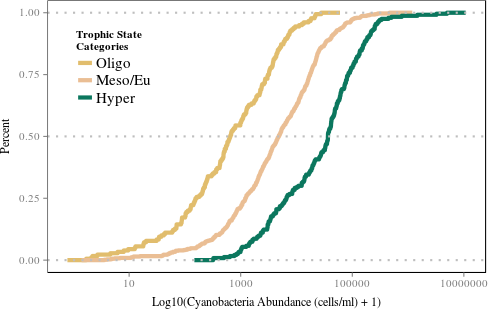
\includegraphics{manuscript_files/figure-latex/ts_3_cyano_cdf-1.jpeg}
\caption{Cumulative distribution function of cyanobacetria abundance for
3 trophic state classes\label{fig:ts_3_cyano_cdf}}
\end{figure}

\newpage

\begin{figure}[htbp]
\centering
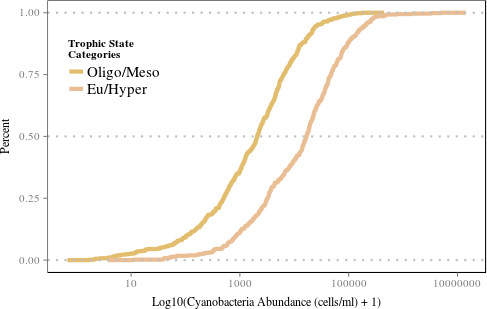
\includegraphics{manuscript_files/figure-latex/ts_2_cyano_cdf-1.jpeg}
\caption{Cumulative distribution function of cyanobacetria abundance for
2 trophic state classes\label{fig:ts_2_cyano_cdf}}
\end{figure}

\newpage

\begin{figure}[htbp]
\centering
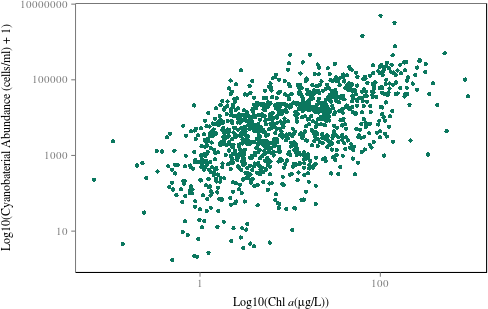
\includegraphics{manuscript_files/figure-latex/scatterplot-1.jpeg}
\caption{Cholorphyll \emph{a} and cyanobacteria abundance
scatterplot\label{fig:scatterplot}}
\end{figure}

\newpage

\section{Tables}\label{tables}

\begin{longtable}[c]{@{}llll@{}}
\caption{Chlorophyll a based trophic state cut-offs with total number of
possible observations.\label{tab:trophicStateTable}}\tabularnewline
\toprule
Trophic State (4 class) & Trophic State (3 class) & Trophic State (2
class) & Concentration Cut-off\tabularnewline
\midrule
\endfirsthead
\toprule
Trophic State (4 class) & Trophic State (3 class) & Trophic State (2
class) & Concentration Cut-off\tabularnewline
\midrule
\endhead
oligotrophic & oligotrophic & oligotrophic/mesotrophic & \textless{}=
0.2\tabularnewline
mesotrophic & mesotrophic/eutrophic & oligotrophic/mesotrophic &
\textgreater{}2-7\tabularnewline
eutrophic & mesotrophic/eutrophic & eutrophic/hypereutrophic &
\textgreater{}7-30\tabularnewline
hypereutrophic & hypereutrophic & eutrophic/hypereutrophic &
\textgreater{}30\tabularnewline
\bottomrule
\end{longtable}

\newpage

\begin{longtable}[c]{@{}llllll@{}}
\caption{Random Forest confusion matrix for Model 1. Columns show
predicted values and rows show observed values. Agreement indicated on
diagonal and accuracy for each trophic state indicated in `Class
Accuracy' column. \label{tab:Confusion_Model1}}\tabularnewline
\toprule
& Oligo & Meso & Eu & Hyper & Class Accuracy\tabularnewline
\midrule
\endfirsthead
\toprule
& Oligo & Meso & Eu & Hyper & Class Accuracy\tabularnewline
\midrule
\endhead
Oligo & 135 & 58 & 4 & 1 & 68\%\tabularnewline
Meso & 42 & 233 & 77 & 10 & 64\%\tabularnewline
Eu & 2 & 66 & 222 & 46 & 66\%\tabularnewline
Hyper & 0 & 3 & 69 & 174 & 71\%\tabularnewline
\bottomrule
\end{longtable}

\newpage

\begin{longtable}[c]{@{}lllll@{}}
\caption{Random Forest confusion matrix for Model 2. Columns show
predicted values and rows show observed values. Agreement indicated on
diagonal and accuracy for each trophic state indicated in `Class
Accuracy' column. \label{tab:Confusion_Model2}}\tabularnewline
\toprule
& Oligo & Meso/Eu & Hyper & Class Accuracy\tabularnewline
\midrule
\endfirsthead
\toprule
& Oligo & Meso/Eu & Hyper & Class Accuracy\tabularnewline
\midrule
\endhead
Oligo & 122 & 74 & 0 & 62\%\tabularnewline
Meso/Eu & 43 & 604 & 42 & 88\%\tabularnewline
Hyper & 0 & 72 & 173 & 71\%\tabularnewline
\bottomrule
\end{longtable}

\newpage

\begin{longtable}[c]{@{}llll@{}}
\caption{Random Forest confusion matrix for Model 3. Columns show
predicted values and rows show observed values. Agreement indicated on
diagonal and accuracy for each trophic state indicated in `Class
Accuracy' column. \label{tab:Confusion_Model3}}\tabularnewline
\toprule
& Oligo/Meso & Eu/Hyper & Class Accuracy\tabularnewline
\midrule
\endfirsthead
\toprule
& Oligo/Meso & Eu/Hyper & Class Accuracy\tabularnewline
\midrule
\endhead
Oligo/Meso & 485 & 75 & 87\%\tabularnewline
Eu/Hyper & 77 & 505 & 87\%\tabularnewline
\bottomrule
\end{longtable}

\newpage

\begin{longtable}[c]{@{}llllll@{}}
\caption{Random Forest confusion matrix for Model 4. Columns show
predicted values and rows show observed values. Agreement indicated on
diagonal and accuracy for each trophic state indicated in `Class
Accuracy' column. \label{tab:Confusion_Model4}}\tabularnewline
\toprule
& Oligo & Meso & Eu & Hyper & Class Accuracy\tabularnewline
\midrule
\endfirsthead
\toprule
& Oligo & Meso & Eu & Hyper & Class Accuracy\tabularnewline
\midrule
\endhead
Oligo & 94 & 72 & 28 & 2 & 48\%\tabularnewline
Meso & 50 & 201 & 80 & 30 & 56\%\tabularnewline
Eu & 21 & 110 & 131 & 73 & 39\%\tabularnewline
Hyper & 1 & 34 & 80 & 131 & 53\%\tabularnewline
\bottomrule
\end{longtable}

\newpage

\begin{longtable}[c]{@{}lllll@{}}
\caption{Random Forest confusion matrix for Model 5. Columns show
predicted values and rows show observed values. Agreement indicated on
diagonal and accuracy for each trophic state indicated in `Class
Accuracy' column. \label{tab:Confusion_Model5}}\tabularnewline
\toprule
& Oligo & Meso/Eu & Hyper & Class Accuracy\tabularnewline
\midrule
\endfirsthead
\toprule
& Oligo & Meso/Eu & Hyper & Class Accuracy\tabularnewline
\midrule
\endhead
Oligo & 80 & 115 & 1 & 41\%\tabularnewline
Meso/Eu & 50 & 585 & 61 & 84\%\tabularnewline
Hyper & 0 & 142 & 104 & 42\%\tabularnewline
\bottomrule
\end{longtable}

\newpage

\begin{longtable}[c]{@{}llll@{}}
\caption{Random forest confusion matrix for Model 6. Columns show
predicted values and rows show observed values. Agreement indicated on
diagonal and accuracy for each trophic state indicated in Class
Accuracy' column. \label{tab:Confusion_Model6}}\tabularnewline
\toprule
& Oligo/Meso & Eu/Hyper & Class Accuracy\tabularnewline
\midrule
\endfirsthead
\toprule
& Oligo/Meso & Eu/Hyper & Class Accuracy\tabularnewline
\midrule
\endhead
Oligo/Meso & 428 & 129 & 77\%\tabularnewline
Eu/Hyper & 147 & 434 & 75\%\tabularnewline
\bottomrule
\end{longtable}

\newpage

\section{Appendix 1. Variable
Definitions}\label{appendix-1.-variable-definitions}

\begin{longtable}[c]{@{}lll@{}}
\toprule
variable\_names & description & type\tabularnewline
\midrule
\endhead
PercentImperv\_3000m & Percent Impervious & GIS\tabularnewline
WaterPer\_3000m & Percent Water & GIS\tabularnewline
IceSnowPer\_3000m & Percent Ice/Snow & GIS\tabularnewline
DevOpenPer\_3000m & Percent Developed Open Space & GIS\tabularnewline
DevLowPer\_3000m & Percent Low Intensity Development &
GIS\tabularnewline
DevMedPer\_3000m & Percent Medium Intensity Development &
GIS\tabularnewline
DevHighPer\_3000m & Percent High Intensity Development &
GIS\tabularnewline
BarrenPer\_3000m & Percent Barren & GIS\tabularnewline
DeciduousPer\_3000m & Percent Decidous Forest & GIS\tabularnewline
EvergreenPer\_3000m & Percent Evergreen Forest & GIS\tabularnewline
MixedForPer\_3000m & Percent Mixed Forest & GIS\tabularnewline
ShrubPer\_3000m & Percent Shrub/Scrub & GIS\tabularnewline
GrassPer\_3000m & Percent Grassland & GIS\tabularnewline
PasturePer\_3000m & Percent Pasture & GIS\tabularnewline
CropsPer\_3000m & Percent Cropland & GIS\tabularnewline
WoodyWetPer\_3000m & Percent Woody Wetland & GIS\tabularnewline
HerbWetPer\_3000m & Percent Herbaceuos Wetland & GIS\tabularnewline
AlbersX & Longitude & GIS\tabularnewline
AlbersY & Latitude & GIS\tabularnewline
LakeArea & Lake Surface Area & GIS\tabularnewline
LakePerim & Lake Perimeter & GIS\tabularnewline
ShoreDevel & Shoreline Development Index & GIS\tabularnewline
DATE\_COL & Date Samples Collected & Water Quality\tabularnewline
WSA\_ECO9 & Ecoregion & GIS\tabularnewline
BASINAREA & Watershed Area & GIS\tabularnewline
DEPTHMAX & Maximum Depth & Water Quality\tabularnewline
ELEV\_PT & Elevation & GIS\tabularnewline
DO2\_2M & Dissolved Oxygen & Water Quality\tabularnewline
PH\_FIELD & pH & Water Quality\tabularnewline
COND & Conductivity & Water Quality\tabularnewline
ANC & Acid Neutralizing Capacity & Water Quality\tabularnewline
TURB & Turbidity & Water Quality\tabularnewline
TOC & Total Organic Carbon & Water Quality\tabularnewline
DOC & Dissolved Organic Carbon & Water Quality\tabularnewline
NH4 & Ammonium & Water Quality\tabularnewline
NO3\_NO2 & Nitrate/Nitrite & Water Quality\tabularnewline
NTL & Total Nitrogen & Water Quality\tabularnewline
PTL & Total Phosphorus & Water Quality\tabularnewline
CL & Chloride & Water Quality\tabularnewline
NO3 & Nitrate & Water Quality\tabularnewline
SO4 & Sulfate & Water Quality\tabularnewline
CA & Calcium & Water Quality\tabularnewline
MG & Magnesium & Water Quality\tabularnewline
Na & Sodium & Water Quality\tabularnewline
K & Potassium & Water Quality\tabularnewline
COLOR & Color & Water Quality\tabularnewline
SIO2 & Silica & Water Quality\tabularnewline
H & Hydrogen Ions & Water Quality\tabularnewline
OH & Hydroxide & Water Quality\tabularnewline
NH4ION & Calculate Ammonium & Water Quality\tabularnewline
CATSUM & Cation Sum & Water Quality\tabularnewline
ANSUM2 & Anion Sum & Water Quality\tabularnewline
ANDEF2 & Anion Deficit & Water Quality\tabularnewline
SOBC & Base Cation Sum & Water Quality\tabularnewline
BALANCE2 & Ion Balance & Water Quality\tabularnewline
ORGION & Estimated Organic Anions & Water Quality\tabularnewline
CONCAL2 & Calculated Conductivity & Water Quality\tabularnewline
CONDHO2 & D-H-O Calculated Conductivity & Water Quality\tabularnewline
TmeanW & Mean Profile Water Temperature & Water Quality\tabularnewline
DDs45 & Growing Degree Days & GIS\tabularnewline
MaxLength & Maximum Lake Length & GIS\tabularnewline
MaxWidth & Maximum Lake Width & GIS\tabularnewline
MeanWidth & Mean Lake Width & GIS\tabularnewline
FetchN & Fetch from North & GIS\tabularnewline
FetchNE & Fetch form Northeast & GIS\tabularnewline
FetchE & Fetch from East & GIS\tabularnewline
FetchSE & Fetch from Southeast & GIS\tabularnewline
MaxDepthCorrect & Estimated Maximum Lake Depth & GIS\tabularnewline
VolumeCorrect & Estimated Lake Volume & GIS\tabularnewline
MeanDepthCorrect & Estimated Mean Lake Depth & GIS\tabularnewline
NPratio & Nitrogen:Phophorus Ratio & Water Quality\tabularnewline
\bottomrule
\end{longtable}

\newpage

\section*{References}\label{references}
\addcontentsline{toc}{section}{References}

\textsc{Breiman, L.} 2001. Random forests. Machine learning 45:5--32.

\textsc{Carlson, R. E.} 1977. A trophic state index for lakes. Limnology
and oceanography 22:361--369.

\textsc{Carvalho, L., C. A. Miller, E. M. Scott, G. A. Codd, P. S.
Davies, and A. N. Tyler}. 2011. Cyanobacterial blooms: Statistical
models describing risk factors for national-scale lake assessment and
lake management. Science of The Total Environment 409:5353--5358.

\textsc{Cohen, J.} 1960. A coefficient of agreement for nominal scales.
Educational and Psychological Measurement 20:37--46.

\textsc{Cutler, D. R., T. C. Edwards Jr, K. H. Beard, A. Cutler, K. T.
Hess, J. Gibson, and J. J. Lawler}. 2007. Random forests for
classification in ecology. Ecology 88:2783--2792.

\textsc{Diaz-Uriarte, R.} 2010. VarSelRF: Variable selection using
random forests. R package version 0.7-3.
http://CRAN.R-project.org/package=varSelRF.

\textsc{D{í}az-Uriarte, R., and S. A. De Andres}. 2006. Gene selection
and classification of microarray data using random forest. BMC
bioinformatics 7:3.

\textsc{Downing, J. A., S. B. Watson, and E. McCauley}. 2001. Predicting
cyanobacteria dominance in lakes. Canadian journal of fisheries and
aquatic sciences 58:1905--1908.

\textsc{Hasler, A. D.} 1969. Cultural eutrophication is reversible.
BioScience 19:425--431.

\textsc{Hollister, J. W.} 2014. Lakemorpho: Lake morphometry in R. R
package version 1.0. http://CRAN.R-project.org/package=lakemorpho.

\textsc{Hollister, J. W., W. B. Milstead, and B. J. Kreakie}. 2014.
LakeTrophicModelling: Package to reproduce Hollister et al. (2014)
Modeling lake trophic state: A data mining approach.

\textsc{Hollister, J. W., W. B. Milstead, and M. A. Urrutia}. 2011.
Predicting maximum lake depth from surrounding topography. PLoS ONE
6:e25764.

\textsc{Hollister, J. W., H. A. Walker, and J. F. Paul}. 2008. CProb: A
computational tool for conducting conditional probability analysis.
Journal of environmental quality 37:2392--2396.

\textsc{Hollister, J., and W. B. Milstead}. 2010. Using gIS to estimate
lake volume from limited data. Lake and Reservoir Management
26:194--199.

\textsc{Homer, C., C. Huang, L. Yang, B. Wylie, and M. Coan}. 2004.
Development of a 2001 national land-cover database for the united
states. Photogrammetric Engineering \& Remote Sensing 70:829--840.

\textsc{Hubert, L., and P. Arabie}. 1985. Comparing partitions. Journal
of classification 2:193--218.

\textsc{Imboden, D., and R. G{ä}chter}. 1978. A dynamic lake model for
trophic state prediction. Ecological modelling 4:77--98.

\textsc{Jones, J., M. Knowlton, D. Obrecht, and E. Cook}. 2004.
Importance of landscape variables and morphology on nutrients in
missouri reservoirs. Canadian Journal of Fisheries and Aquatic Sciences
61:1503--1512.

\textsc{Jones, K. B., A. C. Neale, M. S. Nash, R. D. Van Remortel, J. D.
Wickham, K. H. Riitters, and R. V. O'Neill}. 2001. Predicting nutrient
and sediment loadings to streams from landscape metrics: A multiple
watershed study from the united states mid-atlantic region. Landscape
Ecology 16:301--312.

\textsc{Landis, J. R., and G. G. Koch}. 1977. The measurement of
observer agreement for categorical data. biometrics 33:159--174.

\textsc{Liaw, A., and M. Wiener}. 2002. Classification and regression by
randomForest. R News 2:18--22.

\textsc{Milstead, W. B., J. W. Hollister, R. B. Moore, and H. A.
Walker}. 2013. Estimating summer nutrient concentrations in northeastern
lakes from sPARROW load predictions and modeled lake depth and volume.
PloS one 8:e81457.

\textsc{Paul, J. F., and M. E. McDonald}. 2005. Development of
empirical, geographically specific water quality criteria: A conditional
probability analysis approach 41:1211--1223.

\textsc{Peters, J., B. D. Baets, N. E. Verhoest, R. Samson, S. Degroeve,
P. D. Becker, and W. Huybrechts}. 2007. Random forests as a tool for
ecohydrological distribution modelling. Ecological Modelling
207:304--318.

\textsc{Salas, H. J., and P. Martino}. 1991. A simplified phosphorus
trophic state model for warm-water tropical lakes. Water research
25:341--350.

\textsc{Schindler, D. W., and J. R. Vallentyne}. 2008. The algal bowl:
Overfertilization of the world's freshwaters and estuaries. Page 334.
University of Alberta Press Edmonton.

\textsc{Seilheimer, T. S., P. L. Zimmerman, K. M. Stueve, and C. H.
Perry}. 2013. Landscape-scale modeling of water quality in lake superior
and lake michigan watersheds: How useful are forest-based indicators?
Journal of Great Lakes Research 39:211--223.

\textsc{Smith, V. H.} 1998. Cultural eutrophication of inland,
estuarine, and coastal waters. Pages 7--49 \emph{in} Successes,
limitations, and frontiers in ecosystem science. Springer.

\textsc{Smith, V. H., S. B. Joye, R. W. Howarth, and others}. 2006.
Eutrophication of freshwater and marine ecosystems. Limnology and
Oceanography 51:351--355.

\textsc{Smith, V. H., G. D. Tilman, and J. C. Nekola}. 1999.
Eutrophication: Impacts of excess nutrient inputs on freshwater, marine,
and terrestrial ecosystems. Environmental pollution 100:179--196.

\textsc{USEPA}. 2009. National lakes assessment: A collaborative survey
of the nation's lakes. ePA 841-r-09-001. Office of Water; Office of
Research; Development, US Environmental Protection Agency Washington,
DC.

\textsc{Xian, G., C. Homer, and J. Fry}. 2009. Updating the 2001
national land cover database land cover classification to 2006 by using
landsat imagery change detection methods. Remote Sensing of Environment
113:1133--1147.

\textsc{Yuan, L. L., A. I. Pollard, S. Pather, J. L. Oliver, and L.
D'Anglada}. 2014. Managing microcystin: Identifying national-scale
thresholds for total nitrogen and chlorophyll a. Freshwater Biology
59:1970--1981.

\end{document}